\chapter{Predictive Uncertainty in Decision Trees}
\label{chapter:biqt}
This chapter is largely based on our paper accepted in MICCAI 2016 \cite{tanno2016bayesian}.

A key limitation of the current IQT implementation is the lack of a mechanism to communicate confidence in the predicted target image. High quality training data typically come from healthy volunteers. Thus, performance in the presence of pathology or other effects not observed in the training data is questionable. We expect methods to have high confidence in regions where the method has seen lots of similar examples during training, and lower confidence on previously unseen structures. However, current methods implicitly have equal confidence in all areas. Such an uncertainty characterisation is particularly important in medical applications where ultimately images can inform life-and-death decisions. It is also highly beneficial to downstream image processing algorithms, such as registration or tractography, which can propagate the uncertainty into the output.

In this chapter, we introduce an extension of IQT framework which can simultaneously perform reconstruction and uncertainty quantification over its prediction. We propose an efficient way to incorporate Bayesian inference into the framework and name the new method Bayesian IQT (BIQT). To our knowledge, none of the existing super-resolution \cite{rousseau2008brain,coupe2013collaborative,rueda2013single,wang2014sparse} and image synthesis methods \cite{ye2013modality,jog2015mr,burgos2015robust,wein2008automatic} address the problem of uncertainty estimation. Although many can be cast as \textit{maximum a posteriori} (MAP) optimisation problems, the prohibitive dimensionality or complexity of the posterior distribution (due to non-standard regularisation prior) make the computation of uncertainty intractable or expensive. In contrast, the random forest implementation of the original IQT is amenable to uncertainty estimation thanks to the simple linear model at each leaf node, but the current approach computes \textit{maximum likelihood} (ML) solution. BIQT replaces this ML based inference with Bayesian inference (rather than just MAP) and this allows the uncertainty estimate to reflect unfamiliarity of input data (see Fig. \ref{fig:1D_uncertaintyandSR}).

We demonstrate BIQT through super-resolution of DTI on HCP dataset \cite{sotiropoulos2013advances}, which has sufficient size and resolution to provide training data and a testbed to gauge the baseline performance. We then use clinical data sets from multiple sclerosis (MS) and tumour studies to show the efficacy of the uncertainty estimation in the presence of pathology, not represented in the HCP training data.

\section{Introduction}



\section{Method}
Here we first review the original IQT framework based on a regression forest. We then introduce our Bayesian extension, BIQT, highlighting the proposed efficient hyperparameter optimisation method and the robust uncertainty measure. 

\subsection{Background: Image Quality Transfer}
IQT splits a LR image into small patches and performs quality enhancement on them independently. This patch-wise reconstruction is formulated as a regression problem of learning a mapping from each patch $\mathbf{x}$ of $N_l$ voxels in the LR image to a corresponding patch  $\mathbf{y}(\mathbf{x})$ of $N_h$ voxels in the HR image. Input and output voxels are vector-valued containing $p_l$ and $p_h$ values, and thus the mapping is $\mathbf{x}\in\mathbf{R}^{N_lp_l} \rightarrow \mathbf{y}(\mathbf{x})\in\mathbf{R}^{N_hp_h}$. Training data comes from high quality data sets, which are artificially downsampled to provide matched pairs of LR and HR patches. For application, each patch of a LR image is passed through the learned mapping to obtain a HR patch and those patches combine to estimate a HR image. 

\subsection{Background: Decisions Trees and Random Forest}
To solve the above regression problem, IQT employs a variant of random forests \cite{breiman2001random}. The method proceeds in two stages: training and prediction. 
%
% Forest training
%
During training, we grow a number of trees on different sets of training data. Each tree implements a piecewise linear regression; it partitions the input space $\mathbf{R}^{N_lp_l}$ and performs regressions in respective subsets. Learning the structure of a tree on dataset $\mathcal{D}  = \{\mathbf{x}_i, \mathbf{y}_i\}_{i}^{|\mathcal{D}|}$ aims to find an `optimal' sequence of the following form of binary partitioning. At the initial node (root), $\mathcal{D}$ is split into two sets $\mathcal{D}_{\text{R}}$ and $\mathcal{D}_{\text{L}}$ by thresholding one of $J$ scalar functions of $\mathbf{x}$, or \textit{features}, $f_1,...,f_J$. The optimal pair of a feature $f_m$ and a threshold $\tau$ with the most effective splitting is selected by maximising the \textit{information gain} \cite{criminisi2013decision}, $\text{IG}(f_m, \tau,\mathcal{D}) \delequal |\mathcal{D}|\cdot H(\mathcal{D}) - |\mathcal{D}_\text{R}|\cdot H(\mathcal{D}_\text{R}) - |\mathcal{D}_\text{L}|\cdot H(\mathcal{D}_\text{L})$
where  $|\mathcal{D}|$ denotes the size of set $\mathcal{D}$ and $H(\mathcal{D})$ is the average differential entropy of the predictive distribution $\text{P}(\textbf{y}|\textbf{x}, \mathcal{D}, \mathcal{H})$ given by
\begin{equation}\label{eq:meanentropy}
H(\mathcal{D}) \delequal -\frac{1}{|\mathcal{D}|}\sum_{\mathbf{x}\in \mathcal{D}} \int\text{P}(\textbf{y}|\textbf{x}, \mathcal{D}, \mathcal{H})\cdot\text{log} \ \text{P}(\textbf{y}|\textbf{x}, \mathcal{D}, \mathcal{H})\ \mathbf{dy}.
\end{equation}
Maximising the information gain helps selecting the splitting with highest confidence in predictive distributions. This optimization problem is solved by performing golden search on the threshold for all features. The hypothesis space $\mathcal{H}$ specifies the class of statistical models and governs the form of predictive distribution. In particular, IQT fits the ML estimation of a linear model with a Gaussian noise. To control over-fitting, a validation set $\mathcal{D}^{\text{V}}$ with similar size to $\mathcal{D}$ is used and the root node is only split if the residual error is reduced. This process is repeated in all new nodes until no more splits pass the validation test. 

At the time of prediction, every LR patch $\mathbf{x}$ is routed to one of the leaf nodes (nodes with no children) in each tree through a series of binary splitting learned during training, and the corresponding HR patch is estimated by the mode of the predictive distribution. The forest output is computed as the average of predictions from all trees weighted by the inverted variance of predictive distributions. 


\subsection{BIQT: Locally Bayesian Decision Trees}
Our method, BIQT follows the IQT framework described in chapter $2$ and performs a patch-wise reconstruction using a regression forest. The key difference lies in the choice of $\mathcal{H}$ (eq. \eqref{eq:meanentropy}); we fit a Bayesian linear model \cite{bishop2006pattern} instead of standard linear regression. We will again assume that each (clean) output is generated from the linear model $\mathbf{W}\mathbf{x}$ and the observed output is generated by the addition of a Gaussian noise. The previously employed \textit{maximum likelihood} (ML) approach just yields a point-estimate for the model parameters $\mathbf{W}$ and we accept it as the `true' parameter of the model although limited available training data $\mathcal{D} = \{\textbf{x}_i, \textbf{y}_i\}_{i=1}^D$ means that parameter estimation is inherently uncertain. For instance, there might well be several candidates for $\mathbf{W}$ whose likelihood are very close to that of the ML estimator $\mathbf{W}_{ML}$, implying that the data at our disposal are not sufficient to specify the value of $\mathbf{W}$; the model would perform almost equally well even if you chose one of these equally good options for $\mathbf{W}$. Therefore, instead of resorting to a single estimate, it would be more sensible to account for the presence of such uncertainty. To this end, we explore possible extensions of the current method in the Bayesian paradigm. By viewing the linear map $\mathbf{W}$ as a random variable, we can compute the estimated predictive distribution $\text{P}(\mathbf{y}|\mathbf{x},\mathcal{D},\mathcal{H})$ by integrating over all possible values of $\mathbf{W}$ according to their corresponding strength of belief given the data.  One of the limitations of the previous approach is the fact that the covariance of the predictive distribution $\text{P}(\mathbf{y}|\mathbf{x},\mathcal{D}, \mathcal{H})$ is solely determined by the training data $\mathcal{D}$ and fixed for all new test input $\mathbf{x}$. This is not realistic -- for example if the test input is very far from the cloud of training data, you should expect higher uncertainty. We shall see that this Bayesian extension yields an adaptive covariance which varies with the new test input $\mathbf{x}$ in an intuitive manner (Figure \ref{fig:1D_uncertaintyandSR}). 
	
\begin{figure}
 \centering
\includegraphics[width=11.5 cm]{chapter_2/1dBayLinReg.png}
\caption{1D illustration (i.e. both $\mathbf{x}, \mathbf{y} \in \mathbf{R}$ ) of maximum likelihood and Bayesian linear models fitted to the data (blue circles). The red line and shaded areas show the mode and variance (uncertainty) of $\text{P}(\mathbf{y}|\mathbf{x}, \mathcal{D},\mathcal{H})$ at respective $\mathbf{x}$ values. Bayesian method assigns high uncertainty to an input distant from the training data whilst the ML's uncertainty is fixed.}		\label{fig:sample}
\end{figure}
	
	More formally, given an arbitrary subset of training data $\mathcal{D} = \{\mathbf{x}_i, \mathbf{y}_i\}_{i=1}^{N}$ at one of the internal nodes of a tree, Bayesian linear regression fits the model $\mathbf{y} = \mathbf{W}\mathbf{x} + \boldsymbol{\eta}$ where the additive noise $\boldsymbol{\eta}$ and the linear transform $\mathbf{W} \in \mathbf{R}^{N_hp_h\times N_lp_l}$ follow isotropic Gaussian distributions $\text{P}(\boldsymbol{\eta}| \beta) = \mathcal{N}(\boldsymbol{\eta}|\mathbf{0},\beta^{-1}\mathbf{I})$ 
	and $\text{P}(\mathbf{W}_{|}| \alpha) = \mathcal{N}(\mathbf{W}_{|}|\mathbf{0},\alpha^{-1}\mathbf{I})$, with $\mathbf{W}_{|}$ denoting the row-wise vectorised version of $\mathbf{W}$. The hyperparameters $\alpha$ and $\beta$ are positive scalars which will be specified in a data-driven manner (see section \ref{sec:hyperpara}), and $\mathbf{I}$ denotes an identity matrix. The key difference with the previous model is the prior distribution defined on the model parameters $\mathbf{W}$ (see Table \ref{tab:regressioncomparison} for a comparison), which allows us to integrate over all possible candidates of $\mathbf{W}$ in computing the predictive distribution $\text{P}(\mathbf{y}|\mathbf{x}, \mathcal{D},\alpha,\beta )$ in lieu of resorting to a `best' point estimate. Assuming the noise isotropy is equivalent to assuming all the output dimensions are statistically independent with the same variance, which is very unrealistic, and failing to capture correlational structures would be detrimental to the final forest estimate (eq. \ref{eq:finalestimate}). However, applications in DT-SR and parameter mapping confirm that random-forest regression confers only a marginal improvement over decision trees, and so the isotropy assumption should not harm the prediction accuracy too much (although this claim needs attested). As a first attempt at this, we keep the implementation as simple as possible. 
	
	Assuming for now that hyperparameters $\alpha, \beta$ are known, the predictive distribution is computed by marginalising out the model parameters $\mathbf{W}$ as
	\begin{align}
	\text{P}(\mathbf{y}|\mathbf{x}, \mathcal{D},\alpha,\beta ) 
	& = \int \text{P}(\mathbf{y}|\mathbf{x},\alpha,\beta,\mathbf{W}) \cdot \text{P}(\mathbf{W}_{|}|\mathcal{D},\alpha,\beta,) \,\mathbf{dW}\\
	& = \int \text{P}(\mathbf{y}|\mathbf{x},\alpha,\beta,\mathbf{W}) \cdot \frac{\text{P}(\mathbf{Y}|\mathbf{X},\mathbf{W},\alpha,\beta)\text{P}(\mathbf{W}_{|})}{\text{P}(\mathbf{Y}|\mathbf{X},\alpha,\beta)} \,\mathbf{dW}\\
	& = \int \mathcal{N}(\mathbf{y}| \mathbf{W}\mathbf{x},\beta^{-1}\mathbf{I}) \cdot \mathcal{N}(\mathbf{W}_{|}| \beta(\mathbf{YX}^{T}\mathbf{A}^{-T})_{|},\,\oplus_{i=1}^H \mathbf{A}^{-1})\,\mathbf{dW}\\
	&=  \mathcal{N}(\mathbf{y}| \,\mathbf{W}_{\text{Pred}}\mathbf{x},\, \sigma_{\text{Pred}}^2(\mathbf{x})\cdot \mathbf{I} ) \label{eq:baypredictive}
	\end{align}
	where the $i^{\text{th}}$ columns of matrices $\mathbf{X}$ and $\mathbf{Y}$ are given by $\textbf{x}_i$ and $\textbf{y}_i$, the mean linear map $\mathbf{W}_{\text{Pred}} = \mathbf{Y}\mathbf{X}^T\big{(}\mathbf{X}\mathbf{X}^T+\frac{\alpha}{\beta}\mathbf{I}\big{)}^{-1}$ and the variance $\sigma_{\text{Pred}}^2(\mathbf{x}) = \mathbf{x}^{T}\mathbf{A}^{-1}\mathbf{x}+\beta^{-1}$ with $\mathbf{A} = \alpha\mathbf{I}+\beta \mathbf{X}\mathbf{X}^{T}$. The mean differential entropy in equation~\eqref{eq:meanentropy} can be computed as $H(\mathcal{D}) = N_hp_h|\mathcal{D}|^{-1}\sum_{\mathbf{x} \in \mathcal{D}}\text{log}(\mathbf{x}^{T}\mathbf{A}^{-1}\mathbf{x}+\beta^{-1})$ (up to additive constants) and so the information gain in eq \ref{eq:infogain_gauss} can be written as 
	\begin{align*}
	\text{IG}(f_m,\tau,\mathcal{D}) = \sum_{\mathbf{x} \in \mathcal{D}}\text{log}(\mathbf{x}^{T}\mathbf{A}(\mathcal{D})^{-1}\mathbf{x}+\beta^{-1}(\mathcal{D})) & - \sum_{\mathbf{x}\in\mathcal{D}_{\text{L}}}\text{log}(\mathbf{x}^{T}\mathbf{A}(\mathcal{D}_{\text{L}})^{-1}\mathbf{x}+\beta^{-1}(\mathcal{D}_{\text{L}})) 
	\\&- \sum_{\mathbf{x} \in \mathcal{D}_{\text{R}}}\text{log}(\mathbf{x}^{T}\mathbf{A}(\mathcal{D}_{\text{R}})^{-1}\mathbf{x}+\beta^{-1}(\mathcal{D}_{\text{R}}))
	\end{align*}
	where multiplicative/additive constants are dropped and $\mathbf{A}(\mathcal{D}), \beta(\mathcal{D})$ denote the dependence on $\mathcal{D}$. 
	
	%
	%Predictive variance
	%
	
	
	The predictive variance $\sigma_{\text{Pred}}^2(\mathbf{x})$ provides an informative measure of uncertainty over the enhanced patch $\mathbf{y}(\mathbf{x})$ by combining two quantities: the degree of noise in the training data, $\beta^{-1}$ and the degree of `familiarity', $\mathbf{x}^{T}\mathbf{A}^{-1}\mathbf{x}$ which measures how different the input patch $\mathbf{x}$ is from the observed data. For example, if $\mathbf{x}$ contains previously unseen features such as pathology, the familiarity term becomes large, indicating high uncertainty. The equivalent measure for the original IQT, however, solely consists of the term, $\beta^{-1}$ determined from the training data, and yields a fixed uncertainty estimate for any new input $\mathbf{x}$  (see Fig.\ref{fig:1D_uncertaintyandSR} (left) and the second row in Table \ref{tab:regressioncomparison}). Once a full BIQT forest $\mathcal{F} =\{T_{i}\}$ is grown, we perform reconstruction in the same way as before. All leaf nodes are endowed with predictive distributions of the form in equation \eqref{eq:baypredictive}. Denoting by $\sigma_{\text{Pred},T_i}^2(\mathbf{x})$ the predictive variance at the node in $i^{\text{th}}$ tree to which $\mathbf{x}$ has traversed, BIQT quantifies the \textit{uncertainty} over the corresponding output as the ensemble average of the predictive variances over trees in the forest $\mathcal{F}$
	
	\begin{equation}
	\langle\sigma^2_{\text{Pred}}(\mathbf{x})\rangle_{\mathcal{F}} = |\mathcal{F}|^{-1}\sum_{T\in \mathcal{F}}\sigma_{\text{Pred},T}^2(\mathbf{x}).
	\end{equation} 

	
	\begin{table}[ht]
		\centering 
		\small 
		\begin{tabular}{|c|c|c|c|}
			\hline  & Maximum likelihood & Bayesian \\ 
			\hline Model & 	$\begin{aligned}
			\text{P}(\boldsymbol{\eta}| \beta) &= \mathcal{N}(\boldsymbol{\eta}|\mathbf{0},\beta^{-1}\mathbf{I})\\
			\text{P}(\mathbf{y}|\mathbf{x}, \mathbf{W}) &=  \mathcal{N}(\mathbf{y}| \mathbf{W}\mathbf{x},\beta^{-1}\mathbf{I})
			\end{aligned}$  & 	$\begin{aligned} 
			\text{P}(\boldsymbol{\eta}| \beta) &= \mathcal{N}(\boldsymbol{\eta}|\mathbf{0},\beta^{-1}\mathbf{I})\\
			\text{P}(\mathbf{W}_{|}| \alpha) & = \mathcal{N}(\mathbf{W}_{|}|\mathbf{0},\alpha^{-1}\mathbf{I})\\
			\text{P}(\mathbf{y}|\mathbf{x}, \mathbf{W}) &=  \mathcal{N}(\mathbf{y}| \mathbf{W}\mathbf{x},\beta^{-1}\mathbf{I})
			\end{aligned}$ \\ 
			
			\hline $\text{P}(\mathbf{y}|\mathbf{x}, \mathcal{D},\mathcal{H})$ 
			& $\begin{aligned} &\mathcal{N}(\mathbf{y}|\mathbf{W}_{ML}\mathbf{x},\beta^{-1}_{ML} ) \end{aligned}$
			
			& $\begin{aligned} &\mathcal{N}(\mathbf{y}|\mathbf{W}_{\text{MAP}}\mathbf{x},\beta^{-1}_{ML} + \mathbf{x}^{T}\mathbf{A}^{-1}\mathbf{x} ) \end{aligned}$\\
			  
			  &$\begin{aligned}
					&\text{where:}\\
				  	&\mathbf{W}_{ML} = \mathbf{Y}\mathbf{X}^T(\mathbf{X} \mathbf{X}^T)^{-1}\\
				  	&\beta_{ML}^{-1} = \frac{1}{N_hp_h|\mathcal{D}|}\sum_{i=1}^{|\mathcal{D}|}||\mathbf{y}_i - \mathbf{W}_{ML}\mathbf{x}_i||^2_2 \\
				  	&\big{(} \mathbf{W}_{ML}, \beta_{ML} = \text{arg max}_{\mathbf{W},\beta}\text{P}(\mathcal{D}|\mathbf{W},\beta)\big{)}
			  \end{aligned}$ 
			  
			  & $\begin{aligned} 
				  &\text{where:}\\
				  &\mathbf{W}_{\text{Pred}} = \mathbf{Y}\mathbf{X}^T\big{(}\mathbf{X}\mathbf{X}^T+\frac{\alpha_{ML}}{\beta_{ML}}\mathbf{I}\big{)}^{-1} \\
				  &\mathbf{A} =  \alpha_{ML}\mathbf{I}+\beta_{ML} \mathbf{X}\mathbf{X}^{T}\\
				  &\alpha_{ML},\beta_{ML} = \text{arg max}_{\alpha,\beta}\text{P}(\mathcal{D}|\alpha,\beta)
	         \end{aligned}$ \\
			\hline
		\end{tabular} 
		\setlength{\abovecaptionskip}{0.5cm}
		\small
		\caption{\label{tab:regressioncomparison}. Comparison of ML and Bayesian linear models with isotropic Gaussian noise .}
		\setlength{\belowcaptionskip}{0.cm}
	\end{table} 
	
	\subsection{Hyperparameter optimisation}\label{sec:hyperpara}
	A priori the hyper-parameters $\alpha$ and $\beta$ are unknown, so we optimise them by maximising the marginal likelihood $\text{P}(\mathcal{D}|\alpha,\beta)$. Since $\mathbf{W}_{\text{Pred}}$ minimises the $\text{L}2$ regularised error, 	
	$$ \sum_{i=1}^{D}||\mathbf{y}_i - \mathbf{W}\mathbf{x}_{i}||^2_2 + \frac{\alpha}{\beta}||\mathbf{W}_{|}||^2_2$$
	 this optimisation procedure can be viewed as a data-driven determination of regularisation coefficient $\alpha/\beta$. Although a closed form for $\text{P}(\mathcal{D}|\alpha,\beta)$ exists, exhaustive search is impractical as we have to solve this problem for every binary splitting (characterised by a feature and a threshold) at all internal nodes of the tree. We thus derive and use the multi-output generalisation of the Gull-Mackay fixed-point iteration algorithm \cite{mackay1992bayesian}
	\begin{align}
	\beta_{\text{new}} &= \frac{1 - \beta_{\text{old}}\cdot |\mathcal{D}|^{-1} \text{trace}(\textbf{A}(\alpha_{\text{old}}, \beta_{\text{old}})^{-1}\mathbf{X}\mathbf{X}^{T}) }{\frac{1}{|\mathcal{D}|N_hp_h}\sum_{j=1}^{N_hp_h}\sum_{i=1}^{|\mathcal{D}|}[y_{ji} - \boldsymbol{\mu}_j(\alpha_{\text{old}}, \beta_{\text{old}})^{T}\mathbf{x}_i]^2} \\
	\alpha_{\text{new}}& = \frac{N_lp_l - \alpha_{\text{old}}\cdot \text{trace}(\textbf{A}(\alpha_{\text{old}}, \beta_{\text{old}})^{-1}) }{\frac{1}{N_hp_h}\sum_{j=1}^{N_hp_h}\boldsymbol{\mu}_j(\alpha_{\text{old}}, \beta_{\text{old}})^{T}\boldsymbol{\mu}_j(\alpha_{\text{old}}, \beta_{\text{old}})}
	\end{align}
	where $\boldsymbol{\mu}_j(\alpha, \beta) = \beta \cdot \mathbf{A}(\alpha,\beta)^{-1}\sum_{i=1}^{D}y_{ji}\mathbf{x}_i$.  Whilst the standard MATLAB optimisation solver (e.g. \texttt{fminunc}) requires at least $50$ times more computational time per node optimisation than for IQT, this iterative method is only average $2.5$ times more expensive, making the Bayesian extension viable. We use this over Expectation Maximisation algorithm (viewing $\mathbf{W}_{|}$ as a latent variable) for its twice-as-fast convergence rate. 
	
	 It is possible define prior distributions $\text{P}(\alpha,\beta)$ on the hyper-parameters (called \textit{hyperprior}), so we can obtain a more general predictive distribution by marginalising them out:
		\begin{equation*}
	\text{P}(\mathbf{y}|\mathbf{x}, \mathcal{D}) 
	= \int \text{P}(\mathbf{y}|\mathbf{x}, \mathcal{D}, \alpha,\beta) \cdot \text{P}(\alpha,\beta|\mathcal{D}) \,d\alpha \,d\beta .
	\end{equation*}
	 However, computing the integral over the hyperparameter posterior $\text{P}(\alpha,\beta|\mathcal{D})$ is numerically challenging and approximations are usually required. Given that every node optimization requires hundreds of hyper-parameter optimisation, adding another layer of expensive approximation such  as variational methods or Monte Carlo sampling may impose too much computational burden. One popular strategy is to specify the MAP estimate of the hyper-parameters i.e. $\text{argmax}_{\alpha,\beta}\text{P}(\alpha,\beta|\mathcal{D})$. The currently employed approach effectively aims to finds MAP estimates with flat hyperprior distributions, indicating no prior knowledge about $\alpha, \beta$ which is a reasonable assumption. 
	
	\section{Experiments and results}
	Here we demonstrate and evaluate BIQT through the SR of DTI. First we describe the formulation of the application. Second, we compare the baseline performance on the HCP data to the original IQT. Lastly, we demonstrate on clinical images of diseased brains that our uncertainty measure highlights pathologies.
	
	\subsection{Testing on HCP dataset.}
	We test BIQT on another set of $8$ subjects from the HCP cohort. To evaluate reconstruction quality, three metrics are used: the root-mean-squared-error of the six independent DT elements (DT RMSE); the Peak Signal-to-Noise Ratio (PSNR); and the mean Structural Similarity (MSSIM) index \cite{wang2004image}. We super-resolve each DTI after downsampling by a factor of $2$, and these quality measures are then computed between the reconstructed HR image and the ground-truth.  BIQT displays highly statistically significant ($p<10^{-8}$) improvements (see Fig. \ref{fig:performance}) on all three metrics over IQT, linear regression methods and a range of interpolation techniques. In addition, trees obtained with BIQT are generally deeper than those of the original IQT.
	\begin{figure}[ht]
		\centering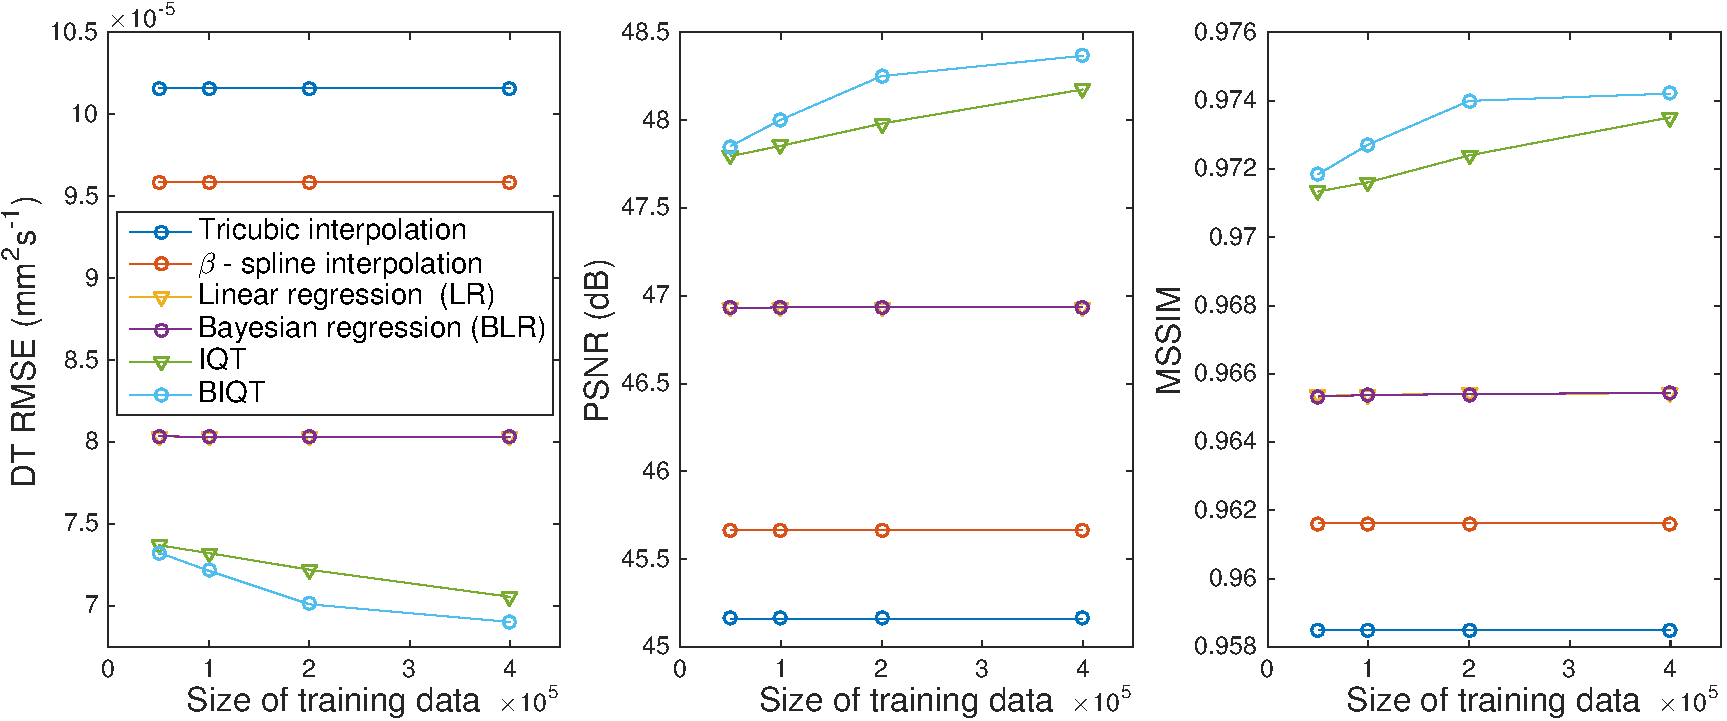
\includegraphics[width= \linewidth]{chapter_2/figure_3.pdf}
		\small 
		\caption{\small Three reconstruction metrics of various SR methods as a function of training data size; RMSE (left), PSNR (middle) and MSSIM (right). The performance of LR (yellow) and BLR (purple) coincide. The results for linear and nearest-neighbour interpolation are omitted for their poor performance.} 
		\label{fig:performance}
	\end{figure}

	Standard linear regression performs as well as the Bayesian regression due to the large training data size. However, with BIQT, as you descend each tree, the number of training data points at each node gets smaller, increasing the degree of uncertainty in model fitting, and so the data-driven regularisation performed in each node-wise Bayesian regression becomes more effective, leading to better reconstruction quality. This is also manifested in the deeper structure of BIQT trees, indicating more successful validation tests and thus greater generalisability. Moreover, BIQT performs reconstruction almost as efficiently as the original IQT, taking only a few minutes for full volume.
			
	\begin{figure}[ht]
		\begin{subfigure}{0.45\textwidth}
			\caption{Maximum Likelihood}
			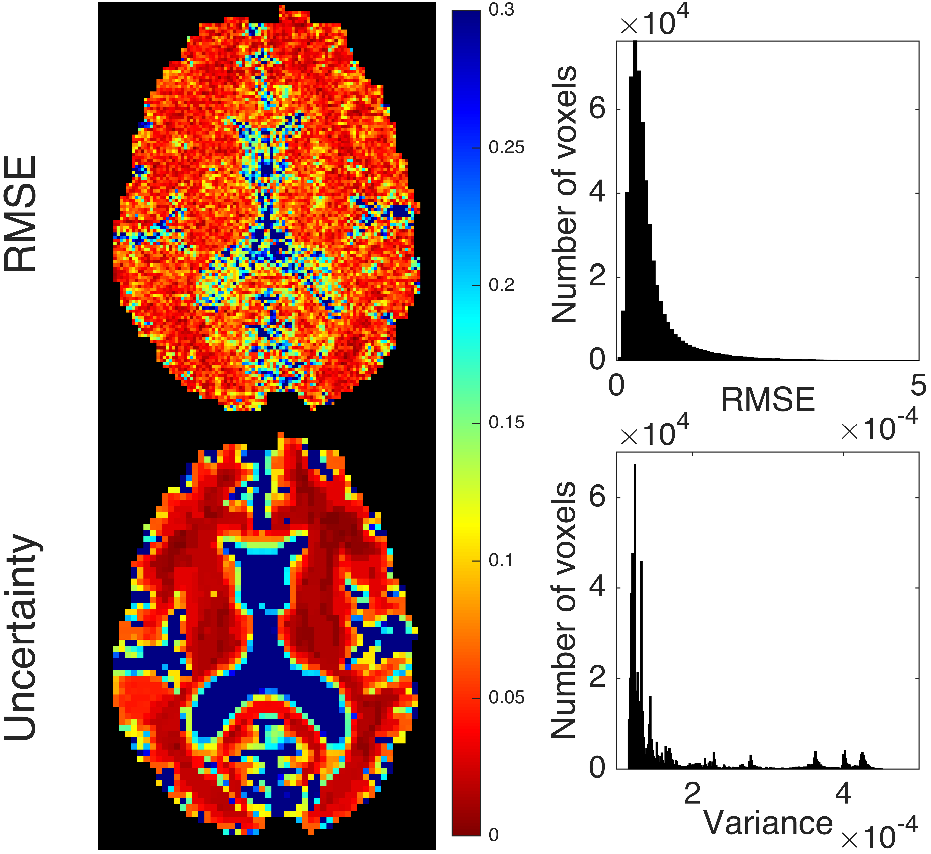
\includegraphics[width=8 cm]{chapter_2/figure_4.pdf}
			\label{fig:map1}
		\end{subfigure}
		\hfill
		\begin{subfigure}{0.43\textwidth}
			\caption{Locally Bayesian RF}
			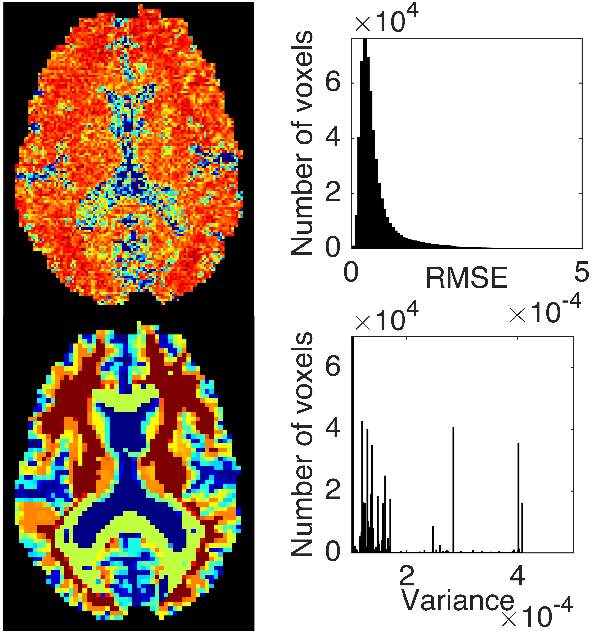
\includegraphics[width=6.9cm]{chapter_2/figure_5.pdf}
			\label{fig:map3}
		\end{subfigure}

%		\subfigure[Original IQT]{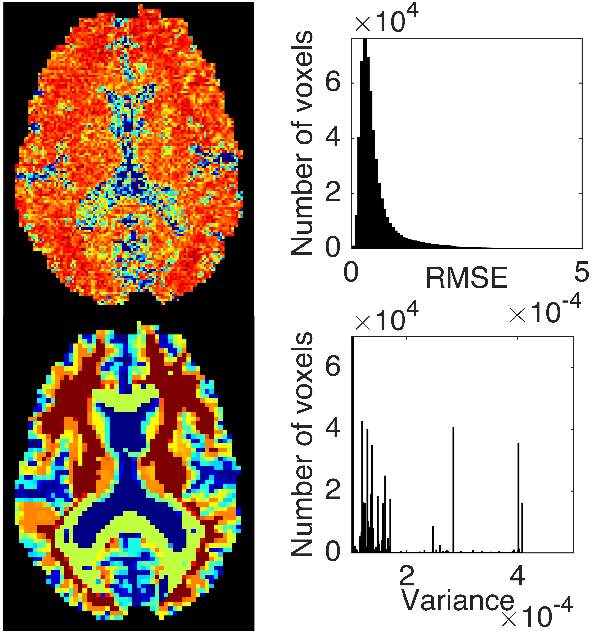
\includegraphics[width=6.9cm]{chapter_2/figure_5.pdf}\label{fig:map3}}
%		%\includegraphics[width=12.cm]{RMSEandConfidMAP_2.pdf}
		\small\caption[Optional caption for list of figures]{ 
			Reconstruction accuracy and uncertainty maps. (top row) The voxel-wise RMSE as a normalised colour-map and its distribution; (bottom row) Uncertainty map (variance) over the super-resolved voxels and its distribution for (a) BIQT and (b) IQT. Trees were trained on $\approx 4\times10^5$ patch pairs.} 
		\label{fig:confidencemap}
		%\vspace{- 10pt}
	\end{figure}

	
	Fig. \ref{fig:confidencemap} shows reconstruction accuracies and uncertainty maps for BIQT and IQT. The uncertainty map of BIQT is more consistent with its reconstruction accuracy when compared to the original IQT. Higher resemblance is also observed between the distribution of accuracy (RMSE) and uncertainty (variance). The BIQT uncertainty map also highlights subtle variations in the reconstruction-quality within the white matter, whereas the IQT map contains flatter contrasts with discrete uncertainties that vary greatly in the same region (see histograms in bottom row). This improvement reflects the positive effect of the data-driven regularisation and better generalisability of BIQT and can be observed particularly in the splenium and genu of the Corpus Callosum, where despite good reconstruction accuracy, IQT assigns higher uncertainty than in the rest of the white matter and BIQT indicates a lower and more consistent uncertainty. Thus, the BIQT uncertainty map displays higher correspondence with accuracy and allows for a more informative assessment of reconstruction quality. 
	%%%that the uncertainty map of BIQT (bottom row) is much more consistent with the reconstruction accuracy (top row) in comparison with that of original IQT. Higher resemblance is also observed between the distributions of accuracy (RMSE) and uncertainty (variance). The BIQT uncertainty map reflects some subtle variations in the reconstruction quality within white matter, whereas IQT simply assigns a fixed uncertainty to the whole region. Whilst IQT assigns high uncertainty to splenium and genu of Corpus Callosum despite high reconstruction accuracy, BIQT correctly indicates low uncertainty. The equivalent uncertainty measure for original IQT is solely determined by the training data and independent of the test input, which results in a discrete set of uncertainty values (fixed for each leave of a tree) as opposed to the continuous values attained by BIQT (compare the histograms in bottom row of figure \ref{fig:confidencemap}). 
	Note that while the uncertainty measure for IQT is governed purely by the training data, for BIQT the uncertainty also incorporates the familiarity of the test data.% (see figure \ref{fig:1D_uncertainty}). 
	
	\subsection{Testing on pathological brains}
	We further validate our method on images with previously unseen abnormalities; we use trees trained on healthy subjects from HCP dataset to super-resolve DTIs of MS and brain tumour patients (10 each). We process the raw data (DWI) as before, and only use $b = 1200 \text{ s/mm}^2$ measurements for the MS dataset and $b = 700 \text{ s/mm}^2$ for the tumour dataset. The voxel size for both datasets is $2^3 \text{ mm}^3$. The MS dataset also contains lesion masks manually outlined by a neurologist. Fig. \ref{fig:sickbrains}(a),(c) middle row shows that the uncertainty map of BIQT precisely identifies previously unseen features (pathologies in this case) by assigning lower confidence than for the remaining healthy white matter. Moreover, in accordance with the reconstruction accuracy, the prediction is more confident in pathological regions than in the cerebrospinal fluid (CSF). This is expected since the CSF is essentially free water with low SNR and is also affected by cardiac pulsations, whereas the pathological regions are contained within the white matter and produce better SNR. Each BIQT tree appropriately sends pathological patches into the `white-matter' subspace and its abnormality is detected there by the `familiarity' term, leading to a lower confidence with respect to the healthy white matter. By contrast, IQT sends pathological patches into the CSF subspace and assigns the fixed corresponding uncertainty which is higher than what it should be. In essence, BIQT enables an uncertainty measure which highly correlates with the pathologies in a much more plausible way, and this is achieved by its more effective partitioning of the input space and uncertainty estimation conferred by Bayesian inference. Moreover, Fig. \ref{fig:sickbrains}(b) shows the superior generalisability of BIQT even in reconstruction accuracy (here SR is performed on downsampled clinical DTIs); the RMSE of BIQT for MS patients is even smaller than that of IQT for healthy subjects. 


	\begin{figure}[ht]
		\centering
		\begin{subfigure}{0.50\linewidth}
			\caption{MS}
			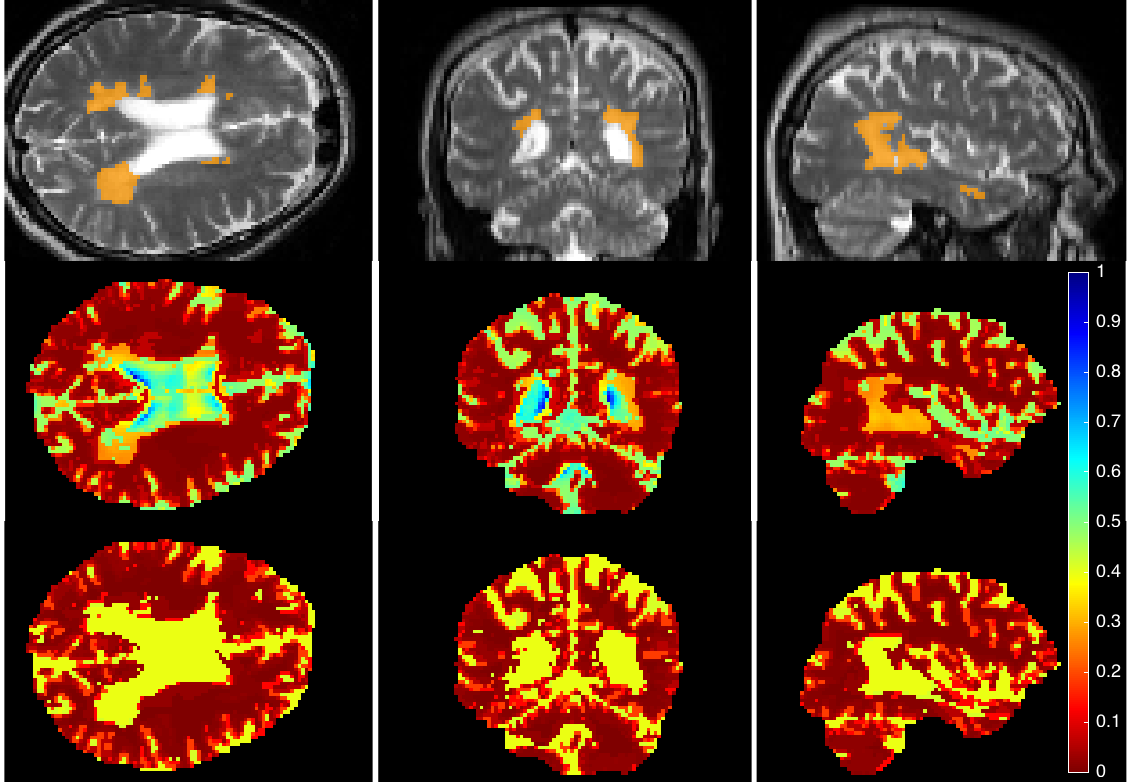
\includegraphics[width=\textwidth]{chapter_2/figure_6.png}
			\label{fig:map1}
		\end{subfigure}
		\begin{subfigure}{0.245\linewidth}
			\caption{RMSE}
			\includegraphics[width=\textwidth]{chapter_2/figure_7.pdf}
			\label{fig:map3}
		\end{subfigure}
   		\begin{subfigure}{0.23\linewidth}
    		\caption{Edema}
    		\includegraphics[width=\textwidth]{chapter_2/figure_8.png}
    		\label{fig:map2}
    	\end{subfigure}
%		\subfigure[MS]\label{fig:map1}}
%		\subfigure[RMSE]{\includegraphics[width=3.7cm]{figure_7.pdf}\label{fig:map3}}
%		\subfigure[Edema]{\includegraphics[width=3.55cm]{figure_8.png}\label{fig:map2}}
		\caption[Optional caption for list of figures]{(a),(c) Normalised uncertainty map (variance is shown i.e. the smaller the more certain) for BIQT (middle row) and IQT (bottom row) along with the T2-weighted slices (top row) for MS (with focal lesions in orange) and edema (contours highlighted), respectively. (b). The RMSE for MS and control subjects (averaged over $10$ subjects in each case).}
		\label{fig:sickbrains}
		%\vspace{-15pt}
	\end{figure}
		
	\section{Summary}
	We presented a computationally viable Bayesian extension of Image Quality Transfer (IQT). The application in super resolution of DTI demonstrated that the method not only achieves better reconstruction accuracy even in the presence of pathology (Fig. \ref{fig:map3}) than the original IQT and standard interpolation techniques, but also provides an uncertainty measure which is highly correlated with the reconstruction quality. Furthermore, the uncertainty map is shown to highlight focal pathologies not observed in the training data. BIQT also performs a computationally efficient reconstruction. Although we have only applied BIQT to DTI-SR, the method preserves the generality of IQT and future work will investigate its performance on tractography and parameter mapping applications. Also, diagnostic values of the method need to be validated in larger-scale experiments.
	
%
%
